\subsection{Por qué la magnetita no se convierte entera}
\label{sec:reduccion-incompleta}

El cuadro~\ref{tab:fases-tiempo} enseña algo que sorprende al leerlo por primera
vez: por mucho que el aglomerado se deje en la mufla a \SI{900}{\celsius},
\textbf{siempre queda magnetita}. A los \SI{150}{\second} el inventario deja de
moverse y ya no cambia hasta los \SI{720}{\second}. No es un artefacto de la
escala ni un residuo numérico: es el resultado, y esta sección explica de dónde
sale.

Conviene mirarlo primero en átomos de hierro y no en masa, porque las fases
pesan distinto y el reparto en masa engaña.

\begin{table}[H]
\centering\small
\begin{tabular}{rrrrrr}
    \hline
     & \multicolumn{5}{c}{\% de los átomos de Fe} \\
    $t$ [s] & en Fe$_2$O$_3$ & en Fe$_3$O$_4$ & en FeO & metálico & en FeTiO$_3$ \\
    \hline
    0 & 12,4 & 81,6 & 0,0 & 0,0 & 6,0 \\
    30 & 12,4 & 81,6 & 0,0 & 0,0 & 6,0 \\
    60 & 0,5 & 93,5 & 0,0 & 0,0 & 6,0 \\
    90 & 0,0 & 89,4 & 4,6 & 0,1 & 6,0 \\
    120 & 0,0 & 81,9 & 10,3 & 1,8 & 6,0 \\
    150 & 0,0 & 75,9 & 14,9 & 3,2 & 6,0 \\
    210 & 0,0 & 75,9 & 14,9 & 3,2 & 6,0 \\
    360 & 0,0 & 75,9 & 14,9 & 3,2 & 6,0 \\
    720 & 0,0 & 75,9 & 14,9 & 3,2 & 6,0 \\
    \hline
\end{tabular}

\caption{Reparto del hierro por fases, en \% de los átomos de Fe presentes. El
\SI{6}{\percent} de la ilmenita no se mueve nunca ---su frontera de reducción
exige \datUmbralIlmenita{}\,\% de CO, que no se alcanza--- y a partir de los
\SI{150}{\second} ninguna fila vuelve a cambiar.}
\label{tab:hierro-reparto}
\end{table}

Se leen tres cosas seguidas. Entre \num{0} y \SI{60}{\second} la hematita
desaparece y la magnetita \emph{crece}, del \num{81.6} al
\SI{93.5}{\percent}: la primera reducción que ocurre no es la de la magnetita,
sino la que la produce, $3\,\mathrm{Fe_2O_3} + \mathrm{CO} \rightarrow
2\,\mathrm{Fe_3O_4} + \mathrm{CO_2}$. Entre \num{60} y \SI{150}{\second} la
magnetita cede el \datMagnetitaConvertida\,\% de lo que llegó a tener, y
aparecen la wüstita y una pizca de hierro metálico. Y a partir de
\SI{150}{\second} no pasa nada más.

\paragraph{No se para por falta de tiempo ni por falta de reductor.} Ésa es la
explicación intuitiva y es la equivocada. El cuadro~\ref{tab:balance-reductor}
hace el balance completo.

\begin{table}[H]
\centering\small
\begin{tabular}{lrl}
    \hline
    Magnitud & Valor & Unidad \\
    \hline
    Magnetita en su máximo (t $=$ 65\,s) & 0,956 & \si{\milli\mol} \\
    Magnetita al final & 0,772 & \si{\milli\mol} \\
    \quad convertida & 0,184\ (19\,\%) & \si{\milli\mol} \\
    Wüstita al final & 0,454 & \si{\milli\mol} \\
    Hierro metálico al final & 0,098 & \si{\milli\mol} \\
    \textbf{O para pasar toda la magnetita a wüstita} & 0,956 & \si{\milli\mol} \\
    \textbf{O que de hecho se quitó} & 0,282\ (30\,\%) & \si{\milli\mol} \\
    Volátil liberado & 233,0 & \si{\milli\gram} \\
    \textbf{CO + H$_2$ generados} & 7,93 & \si{\milli\mol} \\
    \quad frente a lo necesario & $\times$8,3 & --- \\
    \quad \ojo{fracción que llegó a reducir} & 3,6\,\% & --- \\
    \hline
\end{tabular}

\caption{Balance del poder reductor. El carbón genera
\textbf{\datReductorExceso\ veces} más CO$+$H$_2$ del que haría falta para
pasar toda la magnetita a wüstita, y aun así sólo se quita el
\datOxigenoQuitado\,\% del oxígeno. El reductor no es lo que falta.}
\label{tab:balance-reductor}
\end{table}

El carbón libera \datVolatilLiberado\ \si{\milli\gram} de volátil, que en el
reparto de la pirólisis aportan \datReductorGenerado\ \si{\milli\mol} de
CO más H$_2$. Para arrancarle un oxígeno a cada una de las
\datMagnetitaPico\ \si{\milli\mol} de magnetita del máximo harían falta
\datMagnetitaPico\ \si{\milli\mol} de reductor. Hay \datReductorExceso\ veces
más de lo necesario. Y sin embargo sólo el \datReductorAprovechado\,\% de ese
reductor llega a reducir un óxido: el resto sale por el venteo sin haber
reaccionado, con un tiempo de residencia por debajo del segundo.

\paragraph{Se para porque el gas se sitúa sobre la frontera de fases.} La
reducción de la magnetita no es una reacción que consuma reactivo hasta
agotarlo: es un \textbf{equilibrio}. La reacción
\begin{equation}
  \mathrm{Fe_3O_4} + \mathrm{CO} \;\rightleftharpoons\;
  3\,\mathrm{FeO} + \mathrm{CO_2}
\end{equation}
avanza sólo mientras la razón $x_\mathrm{CO} = p_\mathrm{CO} / (p_\mathrm{CO} +
p_\mathrm{CO_2})$ del gas que baña al grano esté \emph{por encima} del valor de
equilibrio, que a \SI{900}{\celsius} vale \datUmbralMagnetita{}\,\%. Pero cada
paso de la reacción gasta un CO y produce un CO$_2$: la propia reducción
\textbf{empuja el gas hacia abajo}, hacia la frontera. Cuando la toca, la
afinidad $1 - Q/K_\mathrm{eq}$ se anula y la reacción se detiene sola ---con
magnetita todavía presente y con CO todavía disponible.

Es el mismo mecanismo por el que un vaso de agua con hielo se queda en
\SI{0}{\celsius}: no es que se acabe el calor, es que mientras coexistan las dos
fases la temperatura no puede moverse. Aquí, mientras coexistan magnetita y
wüstita, $x_\mathrm{CO}$ no puede subir por encima de
\datUmbralMagnetita{}\,\%. La corrida lo confirma sin que se le imponga por
ninguna parte: la media del lecho acaba en \datCOLechoFinal{}\,\%, justo por
debajo del umbral.

Que sea así tiene una consecuencia experimental directa, y es la razón de que
la prueba del imán salga como sale: \textbf{el aglomerado sigue siendo
magnético porque la termodinámica le impide dejar de serlo}. Pasar de la
wüstita al hierro exigiría un gas mucho más rico, por encima de
\datUmbralWustita{}\,\% de CO, y ese gas el sistema no puede fabricárselo
mientras haya magnetita tamponándolo.

\paragraph{La palanca real es el venteo, y va en el sentido contrario.} Del
balance sale un corolario incómodo para quien quisiera reducir más: como el
\datReductorAprovechado\,\% aprovechado está limitado por el \emph{contacto} y
no por la cantidad, cerrar mejor el crisol ---alargar el tiempo de residencia
del gas--- sí convertiría más magnetita. Es decir, \textbf{sellar el crisol
volvería el producto menos magnético}, no más.

Esto no contradice lo de \S\ref{sec:rutas}: allí la tapa ayuda porque actúa
\emph{al enfriar}, sobre la wüstita ya formada, y aquí estorbaría \emph{en
caliente}, dejando formar más wüstita. Son dos etapas distintas, y el óptimo
para los ensayos de adsorción es \textbf{crisol venteado en caliente y tapado
al enfriar}, que es justo el procedimiento que ya se sigue.

\paragraph{Lo que este razonamiento no cubre.} Todo lo anterior explica por qué
la conversión se detiene, pero \emph{no} explica la discrepancia declarada más
arriba: el laboratorio observa que el magnetismo sigue bajando después de los
\SI{150}{\second} y aquí el inventario ya no se mueve. El balance la agudiza,
de hecho. Si sólo se aprovecha el \datReductorAprovechado\,\% del reductor
generado, el margen para que una regeneración lenta de CO por Boudouard siga
mordiendo durante minutos existe de sobra; lo que falta es la constante que
fije a qué velocidad. No se ha ajustado para cuadrar la observación, y ése es
justamente el punto: sería la cuarta vez que este proyecto mueve una constante
hasta hacer coincidir el número que está mirando.

\begin{figure}[H]
\centering
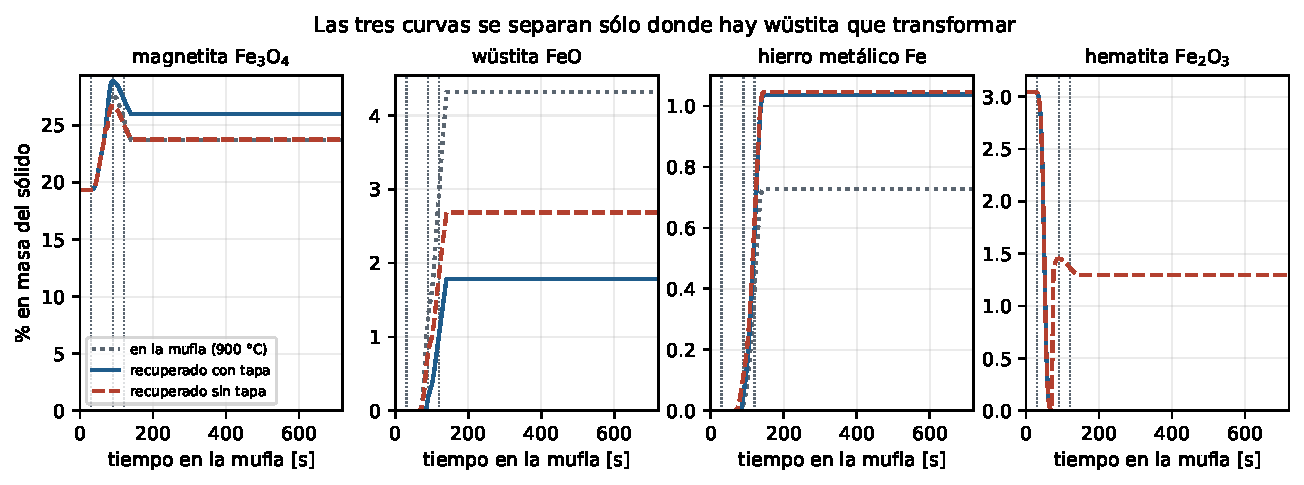
\includegraphics[width=\textwidth]{fig_fen_tres_estados}
\caption{La misma fase en los tres estados en que puede encontrarse: dentro de
la mufla, recuperada tras enfriar con la tapa puesta, y recuperada sin tapa. Las
tres curvas nacen juntas y sólo se separan a partir de los \SI{90}{\second},
cuando aparece la primera wüstita: todo lo que distingue a las tres rutas
---eutectoide, reoxidación por el gas encerrado, oxidación al aire--- actúa
sobre la wüstita o sobre lo que ella produce. Antes de que la haya, enfriar de
una manera o de otra da exactamente el mismo sólido.}
\label{fig:tres-estados}
\end{figure}
